\documentclass{standalone}
\usepackage{tikz}
\usepackage{ctex,siunitx}
\setCJKmainfont{Noto Serif CJK SC}
\usepackage{tkz-euclide}
\usepackage{amsmath}
\usetikzlibrary{patterns, calc,3d}
\usetikzlibrary {decorations.pathmorphing,decorations.pathreplacing,decorations.shapes}
\tikzset{label style/.append style={font=\small}}
\begin{document}
\small
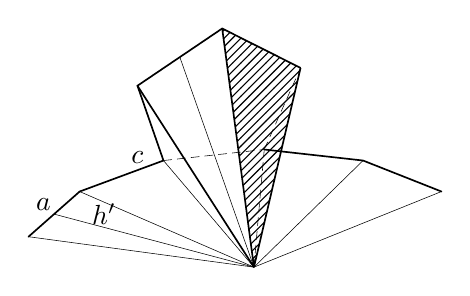
\begin{tikzpicture}[>=latex,scale=1.0,inner sep=1pt,z={(85:5mm)}]
  \begin{scope}[canvas is zx plane at y=0]
    \foreach \x[count=\i from 1] in {A,B,C,D,E,F}
      {\tkzDefPoint(\i*25+260:3){\x}}
    \tkzDefPoints{0/0/S}
    \tkzDefMidPoint(A,B)\tkzGetPoint{M}
    \tkzDrawSegments[semithick](A,B B,C D,E E,F)
    \tkzDrawSegments[densely dashed](C,D S,D)
    \tkzDrawSegments(S,A S,B S,C S,E S,F S,M)
    \tkzLabelLine[pos=0.75,above](S,M){$h'$}
    \tkzLabelLine[pos=0.5,above left](A,B){$a$}
    \tkzLabelLine[pos=0.8,above left](B,C){$c$}
  \end{scope}
  \coordinate (A') at (-0.5019,1.9031,2.2641);
  \coordinate (B') at (-1.5781,1.1762,2.2641);
  \coordinate (N) at (-1.0400,1.5396,2.2641);
  \coordinate (E') at (0.4734,1.1762,2.7189);
  \draw[very thin,densely dashed](D)--(E')--(A')--(B')--(C);
  \draw[semithick](E')--(A')--(B')--(C);
  \draw[semithick](S)--(A')(S)--(B')(S)--(E');
  \draw[very thin](S)--(N);
  \fill[pattern=north east lines](S)--(A')--(E')--cycle;
\end{tikzpicture}
\end{document}